\begin{flushleft}
{\Huge Övriga sånger\\}
\vspace{1cm}
{\Large
Sångförmannen säger:
- Sjung! Sjung på sittningar, sjung på vardagar, sjung idag, sjung
imorgon, sjung för jämnan. Sjung hellre än bra! Här följer en mängd härliga sånger, vissa
med roliga texter, vissa som sjungs vid speciella tillfällen och vissa
som faktiskt är riktigt bra. Håll till godo! 
}
\end{flushleft}

\begin{center}
\vspace{2cm}
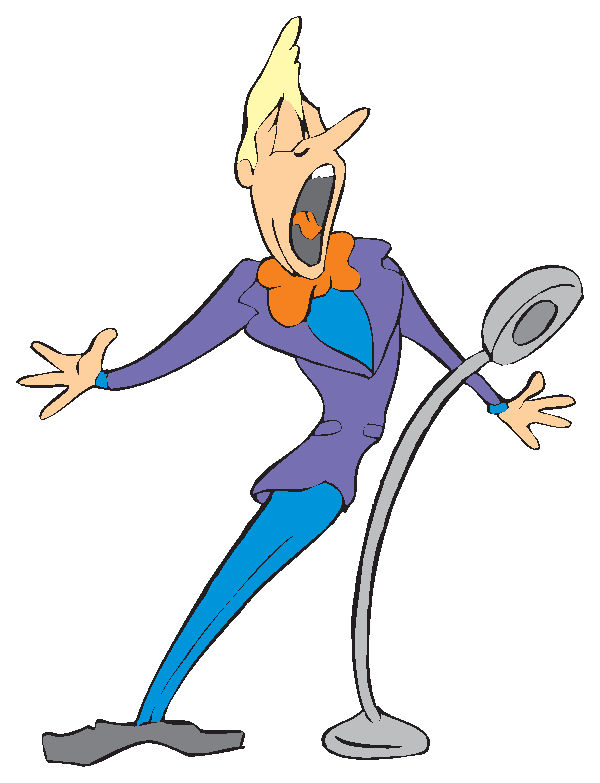
\includegraphics[width=7cm]{bilder/84.eps}
\end{center}

\newpage

\begin{song}{Integralvisan}{integralvisan}
\mel{Med en enkel tulipan}
\begin{vers}
En liten enkel integral\\
i ett vektoranalystal\\
ni har besväret,\\
ni har besväret att derivera.\\
Men tar man Stokes sats däruppå\\
så blir det så enkelt så\\
att integralen, att integralen evaluera.\\
\end{vers}
\begin{vers}
Och rotationen, den integreras\\
sen över ytan utav en boll,\\
koordinaterna transformeras,\\
så integranden blir bara noll.\\
\end{vers}
\begin{vers}
En liten enkel integral\\
i ett vektoranalystal \\
kan va så djävlig\\
att man ej hinner\\
med något mera.\\
\end{vers}
\end{song}

\newpage

%Vers 2 och 3 tillagda av Jas, 2011
\begin{song}{Bär ner mig till sjön}{barnermigtillsjon}
\mel{Bei mir bist du schön}
\begin{vers}
//: Bär ner mig till sjön, bär ner mig till sjön, \\
jag känner att jag måste i. ://\\
Och när du badat mig, så får du torka mig.\\
Och när du torkat mig, så vill jag i igen!\\
Bär ner mig till sjön, bär ner mig till sjön,\\
jag känner att jag måste i.\\
\end{vers}
\begin{vers}
//: Häll i mig en grogg, häll i mig en grogg, \\
jag känner att jag tål det väl. ://\\
Och när jag fått min grogg, så fyll då på igen.\\
Och när du fyllt mitt glas, så häll så i igen!\\
Häll i mig en grogg, häll i mig en grogg,\\
jag känner att jag täl det väl.\\
\end{vers}
\begin{vers}
//: Var var jag igår? Var var jag igår? \\
Jag undrar var jag var igår. ://\\
Mitt huvud känns så tungt, jag kan ej andas lugnt.\\
Hur har jag kommit hem? Vem stoppa mig i säng?\\
Var var jag igår? Var var jag igår?\\
Jag undrar var jag var igår.\\
\end{vers}
\end{song}


\begin{song}{Treo}{treo}
\mel{Vintern rasat}
\begin{vers}
Morgonstund med smak av döda bävrar,\\
frukostmorgonen är över oss.\\
Hur vi stretar, hur vi alla vägrar,\\
så går solen lik förbannat opp.\\
Snart är dagen här med hemska plågor,\\
huvudvärk och ångest, elände, men\\
det finns faktiskt ett glas som kan dig rädda:\\
Treo-comp, vår frälsare och vän.\\
\end{vers}
\end{song}

\newpage

%Tillagd av Jas, 2011
\begin{song}{Dricka alkohol}{drickaalkohol}
\mel{Dansa i neon\\text: Mårten 'Prinzen' Bengtsson, Sandra 'Lilla My' Pettersson}
\begin{vers}
Mitt i en studiedjungel\\
fylld av krav och plugg.\\
Utan mening, utan mål\\
kan inget dugg.\\
\end{vers}
\begin{vers}
Men när natten vaknar\\
tänds ett sista hopp igen\\
och en eld jag saknat.\\
Den flammar upp\\
En gång\\
\end{vers}
\begin{vers}
När vi ska dricka alkohol\\
på vår resa genom natten.\\
Vi ska färdas i ett rus igen\\
vad hände sen?\\
När vi dricker alkohol\\
ända ner till sista slatten.\\
När vi super upp varenda spänn\\
till gryningen.\\
\end{vers}
\begin{vers}
När vi dricker alkohol\\
glömmer bort allt som vi lärt oss.\\
Alla pengar som vi har fått\\
ett minne blott.\\
Vi vill dricka alkohol\\
bara supa inte slåss.\\
Att ha roligt det är inget brott\\
har vi förstått.\\
\end{vers}
\begin{vers}
Så sup med mig.\\
\end{vers}
\end{song}


\begin{song}{Fader Abraham}{faderabraham}
\begin{vers}
Fader Abraham,\\
fader Abraham\\
tio söner hade Abraham\\
och dom åt och drack\\
och dom drack och åt\\
och dom ropa si så här;\\
\end{vers}
\begin{vers}
Höger arm!
\end{vers}
\begin{vers}
Höger arm!, Vänster arm!
\end{vers}
\begin{vers}
...Höger fot! 
\end{vers}
\begin{vers}
...Vänster fot!
\end{vers}
\begin{vers}
...Huvet!  
\end{vers}
\begin{vers}
...Rumpan!
\end{vers}
\begin{vers}
...Tungan!
\end{vers}
\begin{vers}
SKÅL!
\end{vers}
\end{song}

\begin{song}{Fritiof och Carmencita - kort}{fritiof}
	\begin{vers}
		Samborombon, en liten by förutan gata,\\
		som kan dansa tango!\\
	\end{vers}
\end{song}

\newpage

\begin{song}{Nikolajev}{nikolajev}
\mel{Sovjetiska nationalsången}
\begin{vers}
Jag heter Nikolajev\\
och kommer från Sovjet.\\
Jag flyger runt jorden i min rymdraket\\
och jag skall stanna uppe i 84 varv,\\
för det har Chrustjev sagt,\\
men det tycker jag är larv.\\
\end{vers}
\begin{vers}
Jag längtar hem, hem till min planet,\\
till fru och barn, därhemma i Sovjet.\\
Men mest utav allt längtar jag till ett rum,\\
med ett hjärta uppå dörrn.\\
Jag längtar hem till min planet,\\
till fru och barn, där hemma i Sovjet.\\
\end{vers}
\begin{vers}
Min kapsel innehåller många instrument.\\
Ja, mycket av sådant som ännu ej är känt.\\
Men lika förbannat, vad du nu än tror,\\
jag glömde gå på muggen innan jag for.\\
\end{vers}
\begin{vers}
Jag längtar hem ...\\
\end{vers}
\end{song}

\begin{song}{Stockholmsvisan}{stockholmsvisan}
\begin{vers}
Hela Stockholm står i lågor!\\
HURRA, HURRA, HURRA!!!!\\
\end{vers}
\end{song}

\newpage


\begin{song}{Det var i vår ungdom}{detvarivarungdom}
\begin{vers}
Alla:\\
Det var i vår ungdoms fagraste vår\\
vi drack varandra till och vi sade "Gutår!".\\
Och alla så dricker vi nu N.N. till.\\
Solo N.N.:\\
Och N.N. säger inte nej därtill.\\
Alla:\\
Ty, det var i vår ungdoms fagraste vår\\
vi drack varandra till och vi sade "Gutår!".\\
\end{vers}
\end{song}

\newpage

\begin{song}{Brev från kolonien}{brevfrankolonien}
\begin{vers}
Hejsan morsan, hejsan stabben! \\
Här är brev från älsklingsgrabben.\\
Vi har kul på kolonien,\\
vi bor tjugoåtta gangstergrabbar i en...\\
\end{vers}
\begin{vers}
... stor barack med massa sängar. \\
Kan ni skicka mera pengar?\\
För det vore en god gärning,\\
jag har spelat bort vartenda dugg på tärning.\\
\end{vers}
\begin{vers}
Här är roligt vill jag lova, \\
fastän lite svårt att sova.\\
Killen som har sängen över mej\\
han vaknar inte han när han behöver nej.\\
\end{vers}
\begin{vers}
Jag har tappat två framtänder \\
för jag skulle gå på händer\\
när vi lattjade charader,\\
så när morsan nu får se mej får hon spader.\\
\end{vers}
\begin{vers}
Uti skogen finns baciller \\
men min kompis, han har piller\\
som han köpt utav en ful av typ,\\
och om man äter dom blir man en jättekul typ.\\
\end{vers}
\begin{vers}
Jag är inte rädd för spöken, \\
och min kompis han har kröken\\
som han gjort utav potatis\\
och den säljer han i baracken nästan gratis\\
\end{vers}
\begin{vers}
Våran fröken är försvunnen \\
hon har dränkt sig uti brunnen\\
för en morgon blev hon galen\\
för vi släppte ut en huggorm i matsalen\\
\end{vers}
\begin{vers}
Föreståndar'n han har farit \\
han blir aldrig va' han varit,\\
för polisen kom och tog hand\\
om honom för en vecka sedan när vi lekte skogsbrand.\\
\end{vers}
\begin{vers}
Uti skogen finns det rådjur \\
i baracken finns det smådjur,\\
och min bäste kompis Tage\\
han har en liten fickkniv inuti i sin mage.\\
\end{vers}
\begin{vers}
Honom ska dom operera \\
Ja, nu vet jag inge' mera\\
Kram och kyss och hjärtligt tack sen,\\
men nu ska vi ut och bränna grannbaracken!\\
\end{vers}
\end{song}

\newpage

\begin{song}{What shall we do with the drunken sailor}{drunkensailor}
\begin{vers}
What shall we do with the drunken sailor?\\
What shall we do with the drunken sailor?\\
What shall we do with the drunken sailor,\\
early in the morning?\\
\end{vers}
\begin{vers}
Hooray and up she rises.\\
Hooray and up she rises.\\
Hooray and up she rises\\
early in the morning.\\
\end{vers}
\begin{vers}
Put him in the longboat till he's sober...\\
\end{vers}
\begin{vers}
Pull out the plug and wet him all over...\\
\end{vers}
\begin{vers}
Give him a hair of the dog that bit him...\\
\end{vers}
\begin{vers}
Put him in the scuppers with a hose-pipe on him...\\
\end{vers}
\begin{vers}
Heave him by the leg in a runnin' bowline...\\
\end{vers}
\begin{vers}
Shave his head with a rusty razor...\\
\end{vers}
\begin{vers}
Put him in the bed with the captain's daughter...\\
\end{vers}
\begin{vers}
Take him to McDonalds and buy him a burger...\\
\end{vers}
\end{song}

\newpage
%Whiskeysången

%Återinförd av Jas, 2011
\begin{song}{The ball of Kerrymuir}{theballofkerrymuir}
\begin{vers}
There were four-and-twenty virgins\\
coming up from Inverness,\\
and when the ball was over there were\\
four-and-twenty less.\\
\end{vers}
\begin{vers}
Swing your balls to your partner\\
and your arse against the wall.\\
If you don't get fucked on a Saturday night,\\
you'll never get fucked at all.
\end{vers}
\begin{vers}
There was fucking in the kitchen,\\
there was fucking in the halls,\\
you couldn't hear the music\\
for the clanging of the balls.\\
\end{vers}
\begin{vers}
Swing your balls ...\\
\end{vers}
\begin{vers}
The village cripple he was there, he wasn't up too much.\\
He lined them up against the wall,and fucked them with his crutch.\\
\end{vers}
\begin{vers}
Swing your balls ...\\
\end{vers}
\begin{vers}
The village idiot he was there, sitting on a pole.\\
He pulled his foreskin over his head, and whistled through the hole.\\
\end{vers}
\begin{vers}
Swing your balls...\\
\end{vers}
\begin{vers}
Now little Tommy he was there, but he was only eight.\\
He couldn't fuck the women, so he had to masturbate.\\
\end{vers}
\begin{vers}
Swing your balls...\\
\end{vers}
\begin{vers}
The postman, he was also there, the poor man had the pox.\\
He couldn't fuck the lassies, so he fucked the letter-box.\\
\end{vers}
\begin{vers}
Swing your balls...\\
\end{vers}
\begin{vers}
The examinator, he was there, working out a sum;\\
he figured out by logarithms, the time that he would come.\\
\end{vers}
\begin{vers}
Swing your balls...\\
\end{vers}
\begin{vers}
Jock the parson, he was there, it was a bloody shame;\\
loved a lassie thirty times and never knew her name.\\
\end{vers}
\begin{vers}
Swing your balls...\\
\end{vers}
\begin{vers}
Winston Churchill, he was there, down behind the bar,\\
and when he couldn't get it up, he used his big cigar.\\
\end{vers}
\begin{vers}
Swing your balls...\\
\end{vers}
\begin{vers}
And when the ball was over, then everyone confessed.\\
They all enjoyed the music but the fucking was the best!\\
\end{vers}
\begin{vers}
Swing your balls...\\
\end{vers}
\end{song}

%Tillagd av Jas, 2011
\begin{song}{Uti min mage}{utiminmage}
\mel{Uti vår hage}
\begin{vers}
Uti min mage en längtan mig tär,\\
kom hjärtans fröjd.\\
Där råder en en hunger,\\
som ropar så här:\\
Kom kryddsill och kall potatis,\\
kom brännevin quantum satis,\\
kom, allt som kan drickas,\\
kom hjärtans fröjd.\\
\end{vers}
\begin{vers}
Uti min mage en längtan mig tär,\\
kom hjärtans fröjd.\\
Vill du mig något så har jag det där,\\
kom Skåne och Aqua Vitae,\\
kom O.P. och allt vad sprit är,\\
kom ljuva Genever,\\
kom Överste.\\
\end{vers}
\end{song}

\begin{song}{Finsk teknologvisa}{finskteknologvisa}
\mel{Kungliga Södermanlands regementes marsch\\Denna text: Erik Hedman}
\begin{vers}
Här ska ni se ett schack,\\
som aldrig tappar takt, faderalla.
\end{vers}
\begin{vers}
Teknologer vi äro allihop,\\
med vin och kvinnor\\%karlar
vi står på en förtrolig fot.\\
Med tofs i mössan\\
och sticka i vår hand\\
jobba vi flitigt\\
dock helst uti ett vingårdsland.\\
På exkursioner, och fester är vi med.\\
Teolog är man ej\\
och vi tackar vår lycka för de'...\\
\end{vers}
\begin{vers}
//:Var teknolog,\\
han är en vingårdens man.\\ %Hon...dam
Varthelst i staden man såg,\\
där rantar han.\\ %hon
Lustgårdens frukt,\\
den plockar han\\ %hon
med vita handskar på:\\
Korta krikon, långa krikon,\\ %korta bananer, långa bananer
tjocka krikon, trånga krikon\\ %tjocka bananer, många bananer
plockar han med lust\\ %hon
och ett i sänder://\\
\end{vers}
\end{song}
\newpage

%Tillagd av Jas, 2011
\begin{song}{Majdagen}{majdagen}
\begin{vers}
Som en majdag så skön\\
och som solen så varm\\
är den svenske godtemplarens\\
klappande barm\\
\end{vers}
\begin{vers}
Tude lade lude lade lude lade lej. Hej!\\
Tude lade lude lade lude lade lej.\\
Som en majdag...
\end{vers}
\begin{vers}
För till smör, ost och sill\\
och till småvarmt ibland\\
tar den svenske godtemplaren\\
tår uppå tand.\\
\end{vers}
\begin{vers}
Tude lade lude lade lude lade lej. Hej!\\
Tude lade lude lade lude lade lej.\\
För till smör...
\end{vers}
\end{song}
\begin{song}{Chalmeristvisa}{chalmeristvisa}
\mel{Lumberjack song\\Omarbetad version av F-LTH:s Teknologvisa\\
från Sångarstriden 1982.\\}

\begin{vers}
Jag är Chalmerist och helt OK \\
Jag jobbar hårt och jag roar mig\\
Han är Chalmerist och helt OK\\
Han jobbar hårt och han roar sig\\
\end{vers}
\begin{vers}
Teknik är ball \\
Jag kan Pascal\\
Till gasquen vill jag gå\\
Där träffas alla vänner\\
som är från CTH\\
\end{vers}
\begin{vers}
Teknik är ball...\\
För han är Chalmerist...\\
\end{vers}
\begin{vers}
Min mattebok \\
den gör mig klok\\
Jag läser kärnfysik\\
Jag går på föreläsning\\
och älskar juridik.\\
\end{vers}
\begin{vers}
Hans mattebok...\\
Men han är Chalmerist...\\
\end{vers}

\newp

\begin{vers}
Som ekonom,\\
jag blir Fantom.\\
Konkurser gör mig säll.\\
Till flickor blankt jag nekar.\\
Jag älskar ensamcell.\\
\end{vers}
\begin{vers}
(förvånat) Som ekonom han blir Fantom.\\
Konkurser...\\
(ursinningt) NÄÄ, BUU!\\
\end{vers}
\begin{vers}
Men han är Chalmerist...\\
\end{vers}
\end{song}
\begin{song}{Jag fångade en räv en dag}{raven} 
\begin{vers}
Jag fångade en räv en dag\\ 
men räven slank ur näven\\
Lika glad för det är jag\\
men gladast är nog räven\\
\end{vers}
\begin{vers}
Jag träffade en präst i dag\\
men prästen föll i gatan\\
Lika glad för det är jag\\ 
men gladast är nog satan\\
\end{vers}

\begin{vers}
Jag brukar svänga runt i dans\\
men jag har tappat takten\\
jag finner den ej någonstans\\
var kan jag ha förlagt den?\\
\end{vers}

\end{song}
\newpage

\begin{song}{Pelle Jöns}{pellejons}
\begin{vers}
Det var en gång en daggmask,\\
som hette Pelle Jöns.\\
Han var så rädd för skator,\\
han var så rädd för höns.\\
Han var så rädd för letare och metare med burk!\\
Och den som sätter mask på krok\\ 
den kallar han för skurk.\\
\end{vers}
\begin{vers}
En dag sa lilla masken:\\
''Nu borrar jag mig ner,\\
en meter under marken\\
så syns jag inte mer''\\
Där uppe springer letare och metare och höns.\\
De hitta' många maskar, men inte Pelle Jöns!\\
\end{vers}
\end{song}


\begin{song}{Toreador}{toreador}
\mel{Toreadorarian ur Carmen}
\begin{vers}
Jag älskar Chalmers\\
och Chalmers älskar mig,\\
vill du bli rik - Teknisk Fysik!\\
\end{vers}
\end{song}

\newpage

\begin{song}{Änglamark}{anglamark}
\av{Evert Taube}
\begin{vers}
Kalla den änglamarken eller himlajorden om du vill,\\
jorden vi ärvde och lunden den gröna.\\
Vildrosor och blåsippor och lindblommor och kamomill\\
låt dem få leva, de är ju så sköna.\\
\end{vers}
\begin{vers}
Låt barnen dansa som änglar kring lönn och alm,\\
leka tittut mellan blommande grenar.\\
Låt fåglar leva och sjunga för oss sin psalm,\\
låt fiskar simma kring bryggor och stenar.\\
Sluta att utrota skogarnas alla djur!\\
Låt örnen flyga, låt rådjuren löpa!\\
Låt sista älven som brusar i vår natur\\
brusa alltjämt mellan fjällar och gran och fur!\\
\end{vers}
\begin{vers}
Kalla den änglamarken eller himlajorden om du vill,\\
jorden vi ärvde och lunden den gröna.\\
Vildrosor och blåsippor och lindblommor och kamomill\\
låt dem få leva, de är ju så sköna.\\
\end{vers}
\end{song}

\newpage

\begin{song}{Rövarnas visa}{rovarnasvisa}
\kom{ur Kamomilla stad}
\begin{vers}
Nu drar vi ut på rövarstråt.\\
Ja, vi ska ut och röva.\\
Men bara sånt vi kommer åt,\\
och sånt vi kan behöva.\\
Nu är det mörkt kring stad och land,\\
nu sover folk så gott de kan.\\
Då drar vi väg med vår säck och vår spann.\\
Både Kasper och Jesper och Jonatan.\\
\end{vers}
\begin{vers}
Vi drar till Kamomilla stad,\\
till bageributiken.\\
Vi rövar bröd och marmelad\\
så ingen blir besviken.\\
Det händer väl att Jonatan\\
vill ha en polkagris ibland.\\
Men annars så tar vi så lite vi kan\\
både Kasper och Jesper och Jonatan.\\
\end{vers}
\newp
\begin{vers}
Vi vet så väl vad vi skall ha\\
och har så goda nerver.\\
Hos slaktarn tar vi lejonmat\\
och fläsk och köttkonserver\\
och oxfilé är gott minsann\\
och prickig korv gå också an.\\
Men annars så tar vi så lite vi kan,\\
både Kasper och Jesper och Jonatan.\\
\end{vers}
\begin{vers}
Sen behöver vi också guld\\
och tar det om vi kan det\\
och sen när vi tatt säcken full\\
så drar vi hem till landet\\
då är vi hungriga minsann\\
och mat vi lagar åt varann.\\
Men annars så gör vi så lite vi kan,\\
både Kasper och Jesper och Jonatan.\\
\end{vers}
\end{song}

\newpage

\begin{song}{Balladen om den kaxiga myran}{balladkaxigamyran}
\begin{vers}
Jag uppstämma vill min lyra,\\
fast det blott är en gitarr,\\
och berätta om en myra,\\
som gick ut att leta barr.\\
Han gick ut i morgondiset,\\
sen han druckit sin choklad\\
och försvann i lingonriset\\
//:både mätt och nöjd och glad://\\
\end{vers}
\begin{vers}
Det var långan väg att vandra\\
det var långt till närmsta tall.\\
Han kom bort ifrån dom andra\\
men var glad i alla fall.\\
Femti meter ifrån stacken\\
just när solnedgången kom,\\
hitta' han ett barr på marken\\
//:som han tyckte mycket om://\\
\end{vers}
\begin{vers}
För att lyfta fick han stånka,\\
han fick spänna varje lem,\\
men så började han kånka\\
på det fina barret hem.\\
När han gått i fyra timmar\\
kom han till en ölbutelj,\\
han såg allting som i dimma\\
//:bröstet hävdes som en bälg://\\
\end{vers}
\begin{vers}
Den låg kvar sen förra lördan.\\
- Jag skall släcka törsten min,\\
tänkte han och lade bördan\\
utanför och klättra' in.\\
Han drack upp den sista droppen\\
som fanns kvar i den butelj.\\
Och sedan slog han sig för kroppen\\
//:och skrek ut: - Jag är en älg!://\\
\end{vers}
\begin{vers}
- Ej ett barr jag drar till tjället,\\
nu så ska jag tamejfan\\
lämna skogen och i stället\\
vända upp och ner på stan.\\
Men han kom aldrig till staden,\\
något spärrade han stig,\\
en koloss där låg bland bladen\\
//:och vår myra hejdar sig://\\
\end{vers}
\begin{vers}
Den var hiskelig att skåda,\\
den var stor och den var grå,\\
och vår myra skrek: - Anåda,\\
om du hindrar mig att gå!\\
Han for ilsken på kolossen\\
som låg utsträckt i hans väg.\\
Men vår myra kom ej loss sen,\\
//:han satt fast som i en deg://\\
\end{vers}

\newp

\begin{vers}
Sorgligt slutar denna sången.\\
Myran stretade och drog,\\
men kolossen höll'en fången\\
tills han svalt ihjäl och dog.\\
Undvik alkoholens yra:\\
Du blir stursk, men kroppen loj,\\
och om Du är född till en myra\\
//:- brottas aldrig med ett TOY://\\
\end{vers}
\end{song}

\begin{song}{Uti vår hage}{utivarhage}
\vspace{0.5cm}
\begin{vers}
Uti vår hage där växa blå bär,\\ 
kom hjärtans fröjd.\\
Vill du mig något så träffas vi där.\\
Kom liljor och och akvijleja, kom rosor och salivia,\\ 
kom ljuva krusmynta, kom hjärtans fröjd.\\
\end{vers}
\begin{vers}
Fagra små blommor där bjuda till dans,\\
kom hjärtans fröjd.\\
Vill du så binder jag åt dig en krans.\\
Kom liljor och och akvijleja, kom rosor och salivia,\\ 
kom ljuva krusmynta, kom hjärtans fröjd.\\
\end{vers}
\begin{vers}
Kransen den sätter jag sen i ditt hår,\\ 
kom hjärtans fröjd.\\
Solen den dalar, men hoppet uppgår.\\
Kom liljor och och akvijleja, kom rosor och salivia,\\ 
kom ljuva krusmynta, kom hjärtans fröjd.\\
\end{vers}
\end{song}
\newpage

\begin{song}{Schottis på Valhall}{schottispavalhall}
\begin{vers}
Upp och hoppa Tor! Slå på trumman bror!\\
Det är dans uppå Valhall i natt.\\
Uti Fröjas sal står vår asabal.\\
Opp och hoppa fast Odin har spatt.\\
Slå i mera mjöd, det får bli min död.\\
Nej, se där är ju Idun min skatt.\\
Min valkyria kom hit till vår fruktsamhetsrit.\\
Upp och hoppa på Valhall i natt.\\
\end{vers}
\begin{vers}
Höder han hade maskar i magen.\\
Balder dem bota med supar stora.\\
Vred vart väl Ving-Tor, suparna sakna,\\
Brage bråka och Skade hon skrek:\\
\end{vers}
\begin{vers}
Upp och hoppa...\\
\end{vers}
\begin{vers}
Heimdal i hornet blåste och brumma.\\
Loke han låg där i ruset och rulla.\\
Gudarna gorma, feta och fulla.\\
Allfader Odin kräktes och kvad:\\
\end{vers}
\begin{vers}
Upp och hoppa...\\
\end{vers}
\end{song}

\newpage
\begin{song}{Balladen om herr Fredrik Åkare och den söta fröken Cecilia Lind}{balladfredrik}
\begin{vers}
Från Öckerö loge hörs dragspel och bas\\
och fullmånen lyser som var den av glas.\\
Där dansar Fredrik Åkare, kind emot kind\\
med lilla fröken Cecilia Lind.\\
\end{vers}
\begin{vers}
Hon dansar och blundar så nära intill,\\
hon följer i dansen precis vart han vill.\\
Han för och hon följer lätt som en vind.\\
Men säg, varför rodnar Cecilia Lind?\\
\end{vers}
\begin{vers}
Säg var det för det Fredrik Åkare sa:\\
Du doftar så gott, och du dansar så bra.\\
Din midja är smal och barmen är trind.\\
Vad du är vacker, Cecilia Lind!\\
\end{vers}
\begin{vers}
Men dansen tog slut och vart skulle dom gå?\\
Dom bodde så nära varandra ändå.\\
Till slut kom dom fram till Cecilias grind.\\
Nu vill jag bli kysst, sa Cecilia Lind.\\
\end{vers}

\newp

\begin{vers}
Vet hut, Fredrik Åkare, skäms gamla karln!\\
Cecilia Lind är ju bara ett barn.\\
Ren som en blomma, skygg som en hind.\\
Jag fyller snart sjutton, sa Cecilia Lind.\\
\end{vers}

\begin{vers}
Och stjärnorna vandra och timmarna fly\\
och Fredrik är gammal men månen är ny.\\
Ja, Fredrik är gammal men kärlek är blind.\\
Åh, kyss mig igen, sa Cecilia Lind. \\
\end{vers}
\end{song}

\newpage

%Tillagd av Jas, 2011
\begin{song}{En ballad om dagen efter}{dagenefter}
\begin{vers}
Han vaknade så fyllsjuk i ett främmande rum,\\
Aldrig hade Fredrik Åkare känt sig så dum,\\
ty i slafen strax bredvid låg en jäntunge på glid,\\
fröken lind, en stackars flicka både barnslig och stupid.\\
\end{vers}
\begin{vers}
Månens sken och dragspelstoner kan lura en man,\\
för igår när han var full var Cecilia grann,\\
men idag i solens glans, ser hon mest ut som en schimpans,\\
och mot kudden har hon gnidit av sin forna elegans.\\
\end{vers}
\begin{vers}
Vår Fredrik han är gammal men tjejen är ung,\\
han ångrar vad han gjorde och skammen är tung,\\
den blir inte mindre svår, när han straff för otukt får,\\
för Cecilia har ljugit, hon är bara fjorton år...\\
\end{vers}
\end{song}

\begin{song}{Fritiof Anderssons Paradmarsch}{fritiofmarsch}
\begin{vers}
Här kommer Fritiof Andersson, det snöar på hans hatt,\\
han går med sång, han går med spel!\\
Hej, mina lustiga bröder!\\
Det knarrar under klackarna, det är vinternatt.\\
Hej, om du vill, säg bara till,\\
så går vi hem till Söder!\\
O, bugen Er I bylingar i bucklor och batong\\
och ställen Er på sidorna, för gränden den är trång.\\
Där går en här som frös och svalt men segrade ändå,\\
den går med sång, den går med spel till Spanien och Bordeaux.\\
\end{vers}
\begin{vers}
Sultanen av Arabiens land, vid Röda flodens krök,\\
ja tänk vad han blir glad ibland!\\
Hej, mina lustiga bröder!\\
Han eldar under oxarna, han väntar vårt besök.\\
Hej, om du vill, säg bara till,\\
så går vi hem till Söder!\\
O, bugen beduiner i burnus och baldakin\\
och ställ er här på sidorna och bjuden oss på vin.\\
Där går en här som frös och svalt men segrade ändå,\\
den går med sång, den går med spel till Spanien och Bordeaux.\\
\end{vers}

\newp

\begin{vers}
Där dansar konung Farao uti Egyptens land,\\
ja tänk vad han blir glad ibland!\\
Hej, mina lustiga bröder!\\
Han reser upp ett sidentält uppå Saharas sand.\\
Hej, om du vill, säg bara till,\\
så går vi hem till Söder!\\
O, bugen er slavinnor uti slöjor och salopp\\
och ställ er här på sidorna och skåden vår galopp!\\
Där går en här som frös och svalt men segrade ändå,\\
den går med sång, den går med spel till Spanien och Bordeaux.\\
\end{vers}
\begin{vers}
I Cadiz och Kastilien där stannar vi en tid,\\
sen går vi några mil igen!\\
Hej, mina lustiga bröder!\\
Då kommer kung Alfonsius och hälsar från Madrid\\
Hej, om du vill, säg bara till,\\
så går vi hem till Söder!\\
O, bugen barcelonere i barett och bardisan\\
och ställ er här på sidorna - släpp fram vår karavan.\\
Där går en här som frös och svalt men segrade ändå,\\
den går med sång, den går med spel till Spanien och Bordeaux.\\
\end{vers}

\newp

\begin{vers}
Där går en här, där går en hop, en liten, men en god\\
den går i ur, den går i skur!\\
Hej, mina lustiga bröder!\\
Den kräver vin och kyssar och den kräver drakars blod!\\
Hej, om du vill, säg bara till,\\
så går vi hem till Söder!\\
O, bugen er I borgare i Birka och Borås\\
och ställ er här på sidorna. Trumpet och valthorn, blås!\\
Där går en här som frös och svalt men segrade ändå,\\
den går med sång, den går med spel till Spanien och Bordeaux.\\
\end{vers}
\begin{vers}
På vägarna vi vandra och på böljorna vi gå,\\
vi gå med spel, vi gå med sång!\\
Hej mina lustiga bröder!\\
I alla sorters väder som vår Herre hittar på!\\
Hej, om du vill, säg bara till,\\
så går vi hem till Söder!\\
O, buga dig du brusande bölja där vi gå!\\
Vårt skepp är själva Friheten, besättningen är blå!\\
Den seglade och frös och svalt men segrade ändå,\\
den går med sång, den går med spel till Spanien och Bordeaux.\\
\end{vers}
\end{song}

\newpage

\begin{song}{En kungens man}{enkungensman} 
\begin{vers}
Maria går på vägen som leder ner till byn\\
Hon sjunger och hon skrattar åt lärkorna i skyn\\
Hon är på väg till torget för att sälja lite bröd\\
Och solen stiger varm och stor och färgar himlen röd\\
\end{vers}
\begin{vers}
Då möter hon en herre på en häst med yvig man\\
Han säger:\\
- Jag är kungens man så jag tar vad jag vill ha\\
och du är alltför vacker för att inte ha någon man\\
följ med mig in i skogen skall jag visa vad jag kan.\\
\end{vers}
\begin{vers}
Hon tvingas ner i gräset och han tar på hennes kropp\\
Hon slingrar sig och ber honom: För guds skull hålla opp\\
Men riddarn bara skrattar berusad av sin glöd\\
Så hon tar hans kniv och stöter till och riddaren död\\
\end{vers}
\begin{vers}
Dom fängslade Maria och hon stenades för dråp\\
Men minnet efter riddaren det blev firat varje år\\
Ja herrarna blir hjältar men folket det blir dömt\\
Och vi som ser hur allt går till får veta att vi drömt\\
\end{vers}
\end{song}

\newpage

\begin{song}{Balladen om briggen Blue Bird av Hull}{balladbriggen}
\begin{vers}
Det var Blue Bird av Hull\\
Det var Blue Bird en brigg\\
Som med sviktande stumpar stod på\\
Över soten i snöstorm med nerisad rigg\\
Själva julafton sjuttiotvå\\
-Surra svensken till rors, han kan dreja en spak.\\
Ropa skepparn\\
-Allright boys, lös av!\\
Och Karl Stranne från Smögen\\
Blev surrad till rors\\
På Blue Bird som var dömd att bli vrak\\
\end{vers}
\begin{vers}
Han fick Hållö-fyrs blänk\\
Fast av snöglopp och stänk\\
Han stod halvblind\\
Han fick den i lov\\
Och i lä där låg Smögen\\
Hans hem där hans mor\\
Just fått brevet från Middelsborough\\
-Nå vad säger du Karl?\\
-Går hon klar?\\
-Nej, kapten!\\
-Vi får blossa för här är det slut.\\
-Vi har Hållö om styrbord och brott strax i lä.\\
-Ut med ankarna båtarna ut.\\
Men hon red inte upp\\
Och hon fick ett par brott\\
Som tog båten dom hade gjort klart\\
-Jag tror nog, sa Karl Stranne Att far min gått ut.\\
-Emot oss, jag litar på far!\\
\end{vers}
\begin{vers}
-Båt i lä!\\
-Båt i lä!\\
-Det är far, det är vi!\\
-Det är far min från Smögen. Hallå!\\
-Båt i lä! sjöng han ut\\
-Dom är här jumpa i, alle man vi blir bärgade då.\\
\end{vers}
\begin{vers}
Det var Stranne den äldre\\
En viking, en örn\\
Tog sitt renade brännvin\\
Ur vinskåpets hörn\\
Till att bjuda dom skeppsbrutna på\\
-Hur var namnet på skutan?\\
Han sporde och slog\\
Nio supar i spetsiga glas\\
-Briggen Blue bird.\\
Det tionde glaset han tog\\
Och han slog det mot golvet i kras\\
-Sa ni Blue Bird kapten? Briggen Blue Bird av Hull?\\
-Gud i himlen var är då min son?\\
-Var är pojken kapten för vår frälsares skull?\\
Det blev dödstyst bland männen i vrån!\\
\end{vers}
\begin{vers}
Gubben Stranne\\
Tog sakta sydvästen utav\\
-Spara modern kapten, denna kväll.\\
-Nämn ej namnet på briggen som har gått i kvav.\\
-Nämn ej Blue Bird av Hull är ni snäll.\\
Och kaptenen steg opp\\
Han var grå han var tärd\\
Stormen tjöt knappt man hörde hans ord\\
När han sa med självande röst till sin värd\\
-Karl stod surrad och glömdes ombord.\\
\end{vers}
\end{song}

%Grill 2014. Hämtad från cret. Alltså lundare i Val d'Isere.
\begin{song}{Finland}{finland}
\mel{Högt över havet}
\begin{vers}
Finland är Finland och Finland är bra.\\
Dom har en pipeline med sprit från Moskva.\\
Bada Bastu, piska med ris,\\
hacka hål i is.\\
\end{vers}
\begin{vers}
Danmark är Danmark och Danmark är bra.\\
Dom har en jungfru som sitter så bar.\\
Röde pölsor med Tuborg och lök,\\
vi köpte billig krök\\
\end{vers}
\begin{vers}
Norge är Norge och Norge är bra.\\
Dom har den olja som vi vill ha.\\
Dyrt i baren ett jävla pris,\\
klubba säl med is.\\
\end{vers}
\begin{vers}
Island är Island och Island är bra.\\
Kriser, vulkaner och hästar dom har.\\
Jag fiser i geisern vad var det jag sa, valspeck varje dag.\\
\end{vers}
\begin{vers} 
Sverige är Sverige och Sverige är bäst.\\
Ingvar Kamprad han tjänar mest.\\
Ullared, Abba och Absolut,\\
Nu är visan slut.\\
\end{vers}
\end{song}

